\documentclass[zad,zawodnik,utf8]{sinol}

\title{Wóz Strażacki}
\id{woz}
\author{Przemysław Jakub Kozłowski} % Autor zadania
\pagestyle{fancy}
\iomode{stdin}
\konkurs{XII obóz informatyczny}
\etap{olimpijska}
\day{4}
\date{21.01.2016}
\RAM{128}

\usepackage{graphicx}
\graphicspath{ {.} }

\begin{document}
\begin{tasktext}%

Przed hotelem w Serwach znajduje się parking. Parking jest przestrzenią pomiędzy ulicą a płotem oddzielającym hotel od ulicy. Samochody na parkingu zaparkowane są wzdłuż ulicy. Ulica ma określoną długość, a na końcach ulicy (parkingu) rosną drzewa i nie ma możliwości zaparkowania tam samochodu. Na parkingu jest $n$ zaparkowanych samochodów. Każdy samochód ma pewną długość oraz pozycję, na której jest zaparkowany.

Niemądry uczestnik obozu \texttt{ILOCAMP} chciał zrobić dowcip i aktywował alarm przeciwpożarowy w hotelu w Serwach. Nie wiedział, że po aktywowaniu alarmu automatycznie zgłaszana jest informacja do straży pożarnej, a za nieuzasadnione aktywowanie alarmu obowiązują bardzo wysokie kary.

Do hotelu w Serwach przyjechał Wóz Strażacki. Strażak Przemek szybko zorientował się, że niestety na parkingu nie ma wystarczająco dużo miejsca, aby Wóz Strażacki mógł bezpiecznie zaparkować. Przemek postanowił poprzesuwać niektóre samochody wzdłuż parkingu (w przód lub w tył) tak, aby zrobić miejsce dla bardzo długiego Wozu Strażackiego. Niestety przesunięcie samochodu o $1$ metr trwa $1$ sekundę, a pożar musi być ugaszony jak najszybciej, ponieważ rozprzestrzenia się w zatrważającym tempie. Ponadto w jednej chwili może być przesuwany co najwyżej jeden samochód, ponieważ przyjechało tylko dwóch strażaków. W momencie, gdy Jakub będzie przesuwał samochód, Przemek musi kierować Wozem Strażackim.

Strażak Przemek postanowił odpowiednio wybrać miejsce dla Wozu Strażackiego i samochody do przesunięcia tak, aby łączny czas przesuwania był jak najmniejszy. W tym celu wysłał strażaka Jakuba, aby zapisał pozycje i długości wszystkich samochodów zaparkowanych na parkingu. Strażak Jakub wykonał swoje zadanie natychmiastowo i dostarczył potrzebne dane strażakowi Przemkowi. Strażak Przemek jest nie tylko strażakiem, ale również informatykiem, więc szybko obliczył optymalne miejsce zaparkowania Wozu Strażackiego.

Ty jesteś uczestnikiem obozu \texttt{ILOCAMP}, który przygląda się wszystkiemu z okna hotelu. Jeszcze nie wiesz, że jest to fałszywy alarm i obawiasz się, że treści zadań znajdujące się w pokoju kadry zostaną spalone, a dzisiejsze zawody odwołane. Nie możesz doczekać się rozpoczęcia akcji gaśniczej, więc postanowiłeś obliczyć minimalny czas po jakim strażak Przemek będzie mógł przystąpić do gaszenia pożaru. Znasz długość parkingu oraz długości i pozycje wszystkich samochodów, ponieważ wszystko dokładnie zmierzyłeś podczas wczorajszej wyprawy do sklepu, ale niestety nie znasz długości Wozu Strażackiego. Na szczęście to nie jest problem, bo sprawdziłeś w internecie jakie modele wozów strażackich istnieją na świecie i postanowiłeś obliczyć oddzielnie wynik dla każdego z nich.

\medskip
\noindent
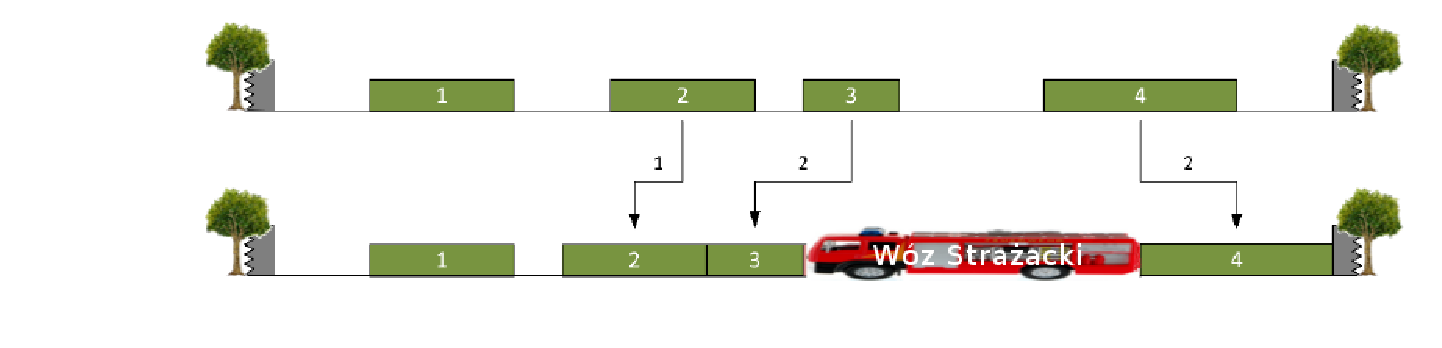
\includegraphics[width=15cm]{rysunek}

  \section{Wejście}
W pierwszym wierszu wejścia znajdują się dwie liczby całkowite $n$ oraz $w$ ($1 \leq n \leq 10^6$, $1 \leq w \leq 10^9$), oznaczające odpowiednio liczbę samochodów na parkingu oraz długość parkingu.

Każdy z kolejnych $n$ wierszy zawiera dwie liczby całkowite $p_i$ oraz $d_i$ ($1 \leq p_i, d_i \leq 10^9$), oznaczające odpowiednio pozycję danego samochodu (odległość bliższej krawędzi samochodu od początku parkingu) oraz długość samochodu. Samochody są podane w kolejności rosnących wartości $p_i$.

Kolejny wiersz zawiera jedną liczbę całkowitą $q$ ($1 \leq q \leq 100$), oznaczającą liczbę modeli wozów strażackich.

Każdy z kolejnych $q$ wierszy zawiera jedną liczbę całkowitą $x_i$ ($1 \leq x_i \leq 10^9$), oznaczającą model wózu strażackiego o długości $x_i$. Modele wozów strażackich są podane w kolejności niemalejących wartości $x_i$.

Możesz dodatkowo założyć, że w testach wartych przynajmniej:\newline
- $40\%$ punktów zachodzi: $n \leq 1000$\newline
- $80\%$ punktów zachodzi: $n \cdot q \leq 10^6$\newline


  \section{Wyjście}
Dla każdego modelu wozu strażackiego należy wypisać jedną liczbę całkowitą -- minimalny czas po jakim taki wóz strażacki mógłby rozpocząć akcję gaśniczą, gdyby przyjechał do Serw. Jeśli ten wóz strażacki nie zmieści się na parkingu nawet po przesunięciu samochodów, to należy wypisać $-1$. Odpowiedzi dla kolejnych modeli należy wypisać w takiej samej kolejności w jakiej wystąpiły na wejściu. Każda odpowiedź powinna znaleźć się w nowej linii.

\makecompactexample

\medskip
\noindent
\textbf{Wyjaśnienie do przykładu:}
Przykład został zilustrowany na rysunku powyżej. Strażak Jakub przesunie samochody $2$ i $3$ w jedną stronę, a samochód $4$ w drugą. Łączenie przesunie samochody o $5$ metrów, więc zajmie mu to $5$ sekund.

\end{tasktext}
\end{document}
